\documentclass[11pt]{article}

\usepackage[margin=1in]{geometry}
\usepackage{parskip}
\usepackage{titlesec}
\usepackage{enumitem}
\usepackage{graphicx}
\usepackage{booktabs}
\usepackage{float}
\usepackage{amsmath}

\titleformat{\section}{\normalfont\large\bfseries}{}{0em}{}
\titlespacing{\section}{0pt}{1.2em}{0.4em}

\title{\vspace{-2em}Final RIT Simulation (ALGO2e) --- Group Write-up}
\author{Group 06\\ \small Alexandre Marthan, Elias Roubache, Elouan Bahri, Jean Jacob, Matthieu Pascal}
\date{\today}

\begin{document}
\maketitle
\vspace{-1em}

\noindent\textbf{Case:} RIT Algorithmic Market Making: Extensions (CNR, RY, AC) \\
\textbf{Account:} Group06\_main \quad\textbar\quad
\textbf{Final P\&L:} \$2,064,738.33 \quad\textbar\quad
\textbf{Fines:} \$0.00

\section{What was our strategy going in?}

The case is built for market making: post a bid and an ask on CNR, RY and AC,
earn the spread plus the limit-order rebate, and keep inventory small. We had
already run a passive market maker, and it lost money. It always quoted both
sides and leaned \emph{against} price moves. When a stock started trending, our
quotes on the losing side kept getting filled, inventory built up in the wrong
direction, and the trend ran us over. That is adverse selection: the orders that
filled us were the informed ones.

For the final simulation we turned that logic around and ran a \textbf{momentum
liquidity taker} (\texttt{last\_simulation.py}):

\begin{itemize}[leftmargin=1.4em, itemsep=0.2em]
  \item \textbf{No limit orders.} The bot only sends MARKET orders, so it never has
        a quote resting in the book to be picked off.
  \item \textbf{Trade with the trend.} For each stock it keeps a 3-tick and a 12-tick
        exponential moving average of the midquote. The trend signal is their
        difference, measured in ticks. Fast above slow means go long; fast below
        slow means go short.
  \item \textbf{Hysteresis.} A position is opened or increased only when
        $|\text{trend}| \ge 1$ tick, and closed when $|\text{trend}| \le 0.3$ tick or
        the trend flips sign. In between, the bot holds. The gap between the two
        thresholds keeps it from flipping back and forth around zero and paying
        fees each time.
  \item \textbf{Fee awareness.} Taking costs \$0.0027/share on CNR and \$0.0015 on
        AC, but on RY you are \emph{paid} \$0.0014/share to take. Adjustments
        under 500 shares are skipped so small rebalances don't eat the edge.
\end{itemize}

\section{What happened during the simulation? Size strategy and script}

\textbf{Ticks 0--210: slow bleed.} For most of the session prices were mostly
noise around a level, with few lasting trends. A 3/12-tick EMA crossover lags by
construction: it buys after a move up, then gets stopped out or exits when the move
reverses. Every round trip also paid the spread and, on CNR and AC, the taker fee.
P\&L drifted down to about $-\$30{,}000$. That is what a momentum taker should
expect when prices tend to revert.

\textbf{Ticks $\approx$210--240: manipulation.} Other participants began pushing
prices hard in one direction, most likely with very large orders that cleared out
the book. To our EMAs this looked like a trend dozens of ticks strong, so the
target size went straight to the 7,000-share cap and the bot traded \emph{with}
the move as it kept going. P\&L jumped from about $-\$30$k to about
\$2{,}000{,}000 within about 30 ticks (Figure~\ref{fig:pnl}). A \$2M gain on at most
21,000 shares (3 stocks $\times$ 7,000) means prices moved by at least
$\$2{,}000{,}000/21{,}000 \approx \$95$ per share. Normal moves in this case are a
few cents, so this jump came from the manipulation, not from our signal having any
edge.

\textbf{Shutting the algorithm off.} When the manipulation stopped, we stopped the
bot by hand. A pushed price usually snaps back once the pushing ends, and a 3/12 EMA
reacts too slowly to get out ahead of that. Running it longer meant either giving
back a large part of the gain or, worse, going short into the snap-back. When we
stopped, one 7,000-share position was still open (left screenshot, P\&L
\$2{,}033{,}518). It was flat by the end of the case, at a final P\&L of
\$2{,}064{,}738 with zero position and no fines (right screenshot).

\begin{figure}[H]
  \centering
  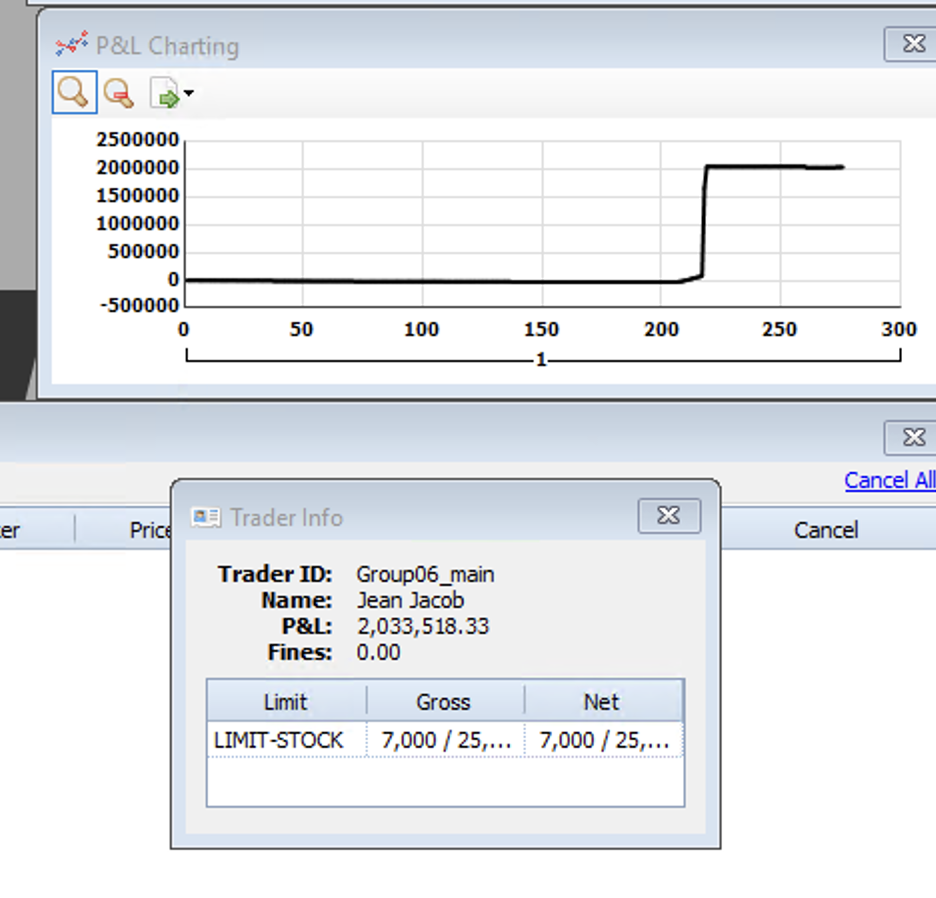
\includegraphics[width=0.42\textwidth]{pnl_open_position.png}\hspace{1.5em}
  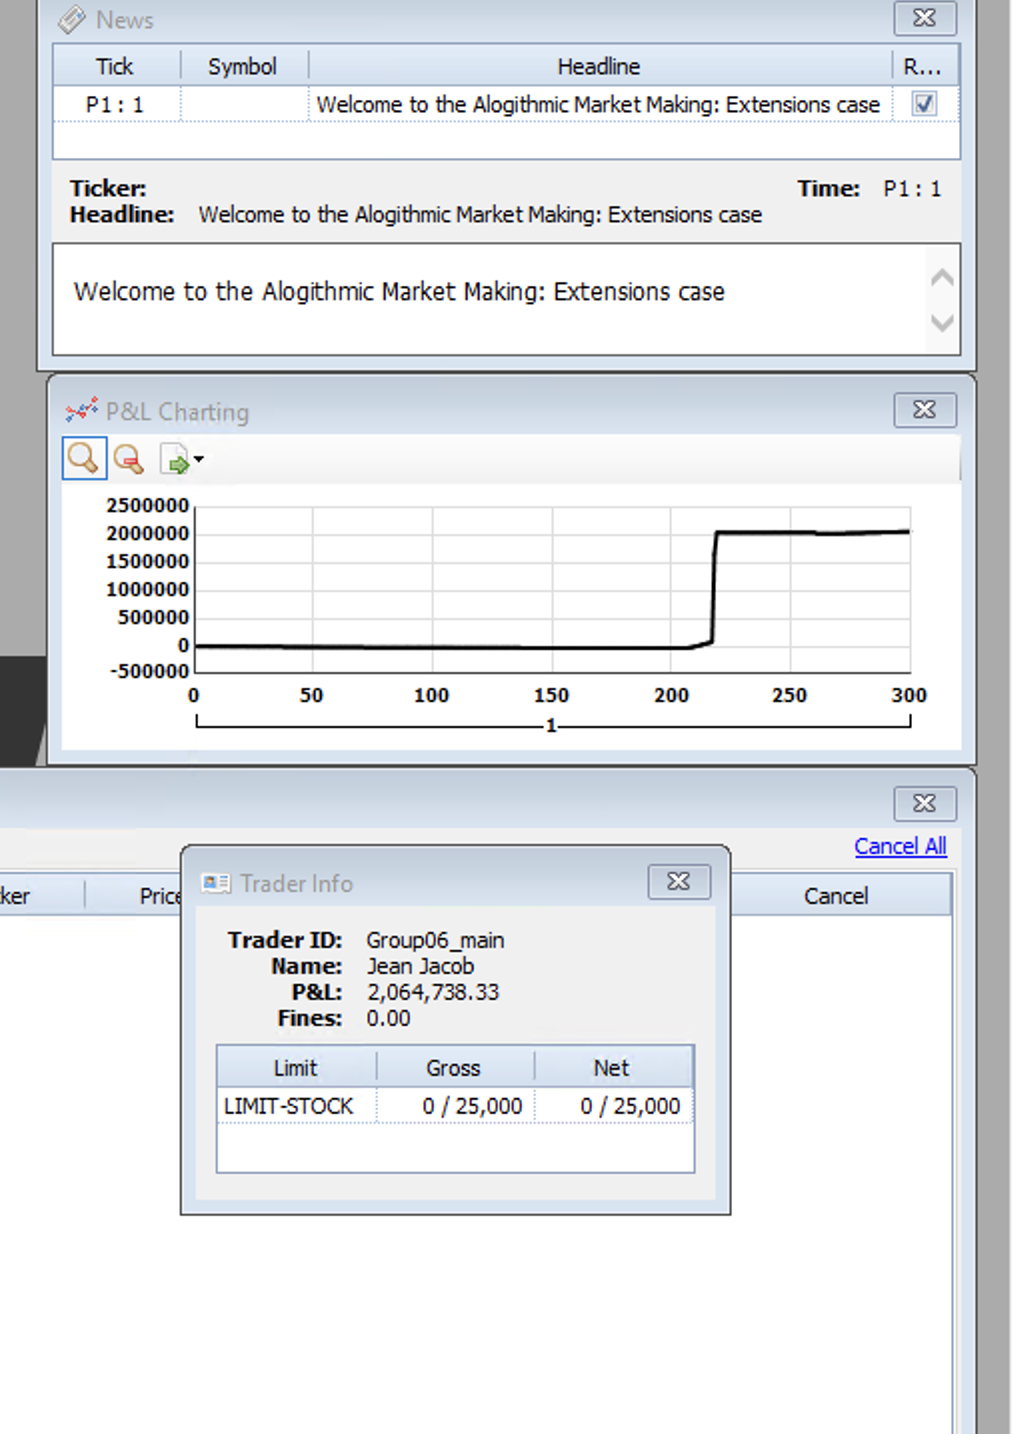
\includegraphics[width=0.36\textwidth]{pnl_final.png}
  \caption{RIT P\&L chart and trader info. Left: shortly after the algorithm was
  stopped, with 7,000 shares still open. Right: end of case, flat.}
  \label{fig:pnl}
\end{figure}

\textbf{Size strategy.} Position size scales with how strong the trend is:
\[
  \text{target}_k = \operatorname{sign}(\text{trend}_k)\cdot
  \min\!\big(7{,}000,\; 2{,}000 \times |\text{trend}_k|\big),
  \quad \text{rounded down to 100 shares.}
\]
A 1-tick trend gives a 2,000-share position; the cap is reached at 3.5 ticks.
Holding 7,000 shares in each of three stocks means at most 21,000 shares gross,
under the 25,000 limit. That is why we were never fined, even with the manipulated
signal maxing out every stock. Orders are capped at 5,000 shares, with at least
0.3\,s between orders on the same stock, because RIT reports positions with a lag.
Risk controls:
\begin{itemize}[leftmargin=1.4em, itemsep=0.2em]
  \item \textbf{Per-stock stop:} if the unrealized loss exceeds 4 ticks per share,
        close the position at market and stay out of that stock for 5\,s.
  \item \textbf{Drawdown breaker:} if total P\&L falls \$1,500 below its peak,
        flatten everything and pause for 30\,s.
  \item \textbf{End of case:} flatten during the last 5 ticks.
\end{itemize}
The drawdown breaker turned out to matter most. Once P\&L reached \$2M, any
\$1,500 pullback would have flattened the book, so the gain was effectively
protected.

\textbf{How to use the script.} Enable the API in the RIT client, then run
\begin{verbatim}
python last_simulation.py --key <API_KEY>
\end{verbatim}
(the default host is \texttt{http://localhost:7238}). It waits for the case to
become ACTIVE, cancels any leftover limit orders, and then trades CNR, RY and AC.
It prints a status line every tick and also writes it to
\texttt{momentum\_log.txt}. Each constant can be overridden on the command line,
e.g.\ \texttt{--max-position 5000 --ema-fast 2 --ema-slow 8 --tickers CNR,AC}. The
script refuses to start if $\text{max-position}\times\#\text{tickers} > 24{,}000$.
Pressing Ctrl+C stops the loop, but it does \emph{not} flatten. Check the RIT
client afterwards and close any position left open, which is what happened to us.

\section{MARKET orders versus LIMIT orders}

\begin{table}[H]
\centering
\small
\begin{tabular}{@{}p{2.4cm}p{6.1cm}p{6.1cm}@{}}
\toprule
 & \textbf{MARKET (our final strategy)} & \textbf{LIMIT (our market maker)} \\
\midrule
Guarantee & Execution, not price & Price, not execution \\
Cost & Pay half the spread plus the taker fee (except RY, which pays a rebate) & Earn the spread plus the rebate \\
Main risk & \emph{Slippage}: in a thin or manipulated book, an order can walk
            several price levels and fill far from the last quote &
            \emph{Adverse selection and inventory}: you fill exactly when the price
            is moving against you, and trends leave you holding the losing side \\
Other risks & Paying spread and fees on every whipsaw in a mean-reverting market &
              Non-execution; being picked off on stale quotes; cancel/replace
              traffic that uses up the API rate limit \\
\bottomrule
\end{tabular}
\end{table}

In this session the two order types lost money for opposite reasons. The market
maker lost because its limit orders gave other traders a free option against it.
The taker lost slowly in the quiet part of the session because it paid the spread
and fees to follow trends that didn't last. The only reason the taker ended
profitable is that the manipulated move was large and one-directional, which is
the one environment momentum strategies are built for. MARKET orders were also the
right tool for that phase: we needed to get into the move, and later out of it,
right away, whatever the fill price. The risk is symmetric, though. The same thin
book that let us ride the push up would have filled our exits at extreme prices if
we had been on the wrong side. The 5,000-share order cap and the 0.3\,s gap between
orders limited how far a single order could walk the book.

\section{What was our P\&L?}

\begin{table}[H]
\centering
\begin{tabular}{@{}lr@{}}
\toprule
Phase & P\&L \\
\midrule
Ticks 0--210 (normal market) & $\approx -\$30{,}000$ \\
After the manipulation, algorithm stopped (7,000 shares open) & \$2{,}033{,}518.33 \\
\textbf{End of case (flat, no fines)} & \textbf{\$2{,}064{,}738.33} \\
\bottomrule
\end{tabular}
\end{table}

\textbf{Takeaways.} We don't treat the \$2M as evidence that the strategy works.
Under normal conditions the momentum taker lost about \$30k. Nearly all of the
gain came from other participants manipulating prices, which would be illegal in
a real market and in any case can't be repeated. What we did get right was the
risk management around that event: hard position caps kept us inside the limits
(no fines), and turning the algorithm off as soon as the manipulation ended
locked in a gain that a lagging trend signal would otherwise have given back. If
we were to keep a strategy for normal conditions, it would be the market maker
with a trend filter: quote passively to earn the spread and rebate, but pull or
skew quotes when the EMA trend signal shows a strong move.

\end{document}
